% Overleaf / GitHub: compile with pdfLaTeX (or XeLaTeX).
% Requires IEEEtran.cls (Overleaf has it; or download from IEEE).
\documentclass[journal,twocolumn,10pt]{IEEEtran}

\usepackage{amsmath,amssymb,amsfonts}
\usepackage{graphicx}
\usepackage{booktabs}
\usepackage{multirow}
\usepackage{xcolor}
\usepackage{cite}
\usepackage{url}
\usepackage{hyperref}
\hypersetup{colorlinks=true,linkcolor=blue,citecolor=blue,urlcolor=blue}

\begin{document}

\title{Hybrid Cost Shaping for Multi-UAV Task Allocation under Delayed Sensing and Perishable Tasks}

\author{
  % Update author block before submission
  Anonymous~Author
  \thanks{Code and experiment scripts accompany this manuscript (Multi-UAV TA Gym environment).}
}

\maketitle

\begin{abstract}
Heterogeneous multi-UAV task allocation is often solved with classical bipartite matching (e.g., the Hungarian method) when the full task set is known and objectives reduce to distance-versus-capability costs.
We show that this myopic optimum weakens under \emph{Windowed Pop-up Strike} (WPS) dynamics: hard time windows, delayed and local sensing, burst arrivals, and attrition.
We propose hybrid allocators that keep Hungarian assignment as the engine while a learned module reshapes task priorities (MLP-RAH and set-attention Att-RAH), trained on a WPS-aligned score \(S_{\mathrm{WPS}}\).
On WPS\_hard (100 episodes), Att-RAH significantly improves \(S_{\mathrm{WPS}}\) over visibility-masked Local-Hungarian (paired bootstrap 95\% CI excludes zero); a Global-Hungarian oracle remains an upper bound.
A harder multi-front suite (WPS\_attn: 12 UAVs, dual-region bursts, no knowledge sharing) widens the oracle gap but does \emph{not} separate Att-RAH from MLP or urgency-only ablations---indicating that under priority-reshape hybrids, information asymmetry dominates architecture.
We release metrics, figures, and training scripts aligned with the reported tables.
\end{abstract}

\begin{IEEEkeywords}
Multi-UAV systems, task allocation, Hungarian algorithm, attention, hybrid learning, time windows, partial observability
\end{IEEEkeywords}

\section{Introduction}
Multi-UAV mission planners routinely cast allocation as bipartite matching between agents and tasks~\cite{kuhn1955hungarian,gerkey2004formal}.
When every UAV observes every task and costs are dominated by travel and capability fit, periodic Hungarian (or auction/CBBA) solvers are strong baselines~\cite{choi2009cbba}.
In that regime, end-to-end reinforcement learning (RL) often \emph{ties} rather than beats classical assignment.

This paper studies a setting where myopic global (or even team-union) matching is the \emph{wrong} inductive bias:
\begin{itemize}
  \item \textbf{Hard windows:} pop-up attack/recon/intercept tasks expire; misses incur explicit penalties.
  \item \textbf{Delayed / local sensing:} new threats are not globally known; each UAV discovers tasks within a sensing radius or after a delay.
  \item \textbf{Burst arrivals:} correlated pop-ups punish greedy over-commitment of the fleet.
\end{itemize}
We call this suite \textbf{WPS} (Windowed Pop-up Strike).
The fair classical competitor is \textbf{Local-Hungarian}: Hungarian matching on open tasks with edges masked by each agent's known-task set.
Omniscient \textbf{Global-Hungarian} is reported only as an information oracle.

Our method is a \textbf{hybrid}: RL (or set attention) predicts per-task priorities and a soft reserve fraction \(\rho\); Hungarian then solves the reshaped cost problem on the same visibility mask.
This preserves a strong combinatorial engine while injecting foresight that pure myopic costs lack.

\paragraph{Contributions.}
(1)~WPS scenarios and a primary metric \(S_{\mathrm{WPS}}\) focused on perishable outcomes;
(2)~MLP-RAH and Att-RAH hybrids with visibility-masked Local-Hungarian;
(3)~100-episode evaluation with paired bootstrap CIs versus Local-Hungarian on WPS\_hard;
(4)~a multi-front attention stress suite (WPS\_attn) showing that set attention does not beat urgency heuristics when the interface remains cost reshaping.

\section{Related Work}
\textbf{Classical allocation.}
The Hungarian algorithm~\cite{kuhn1955hungarian} and market-based CBBA~\cite{choi2009cbba} remain standard for multi-robot TA.
Capability-greedy heuristics provide weak baselines.

\textbf{Learning for TA.}
Attention-based policies over task tokens appear in recent multi-agent TA and routing work; our prior TBTA stack uses multi-head attention DQNs over task embeddings for discrete assignment.
Pure RL, however, struggles when the combinatorial core is bipartite matching under dense costs.

\textbf{Hybrids.}
Combining learned scoring with classical solvers (learning-to-rank / cost shaping) is a recurring theme in operations research and robotics.
We adopt that pattern under partial observability and hard deadlines.

\section{Problem Setting: WPS}
We simulate heterogeneous fleets (fighter/recon types) with static Att/Rec missions plus dynamic threats that spawn relative intercept tasks and online Att/Rec arrivals.
WPS configuration knobs include sensing radius \(R_{\mathrm{sense}}\), threat delay \(d\), window length \(W\), burst size, fail rate, and miss/on-time weights.
Local knowledge is tracked per agent; Local-Hungarian forbids assigning an agent to an unknown task.

Three locked suites plus one attention stress suite are used:
\begin{itemize}
  \item \textbf{WPS\_easy:} larger radius, longer windows, no burst.
  \item \textbf{WPS\_hard:} tighter windows, stronger delay, bursts (main positive claim).
  \item \textbf{WPS\_burst:} stress test with larger bursts and shorter windows.
  \item \textbf{WPS\_attn:} 12 UAVs, scarce F2 specialists, dual-region burst spawn, no team knowledge sharing (attention stress).
\end{itemize}

\section{Methods}
\subsection{Baselines}
\textbf{Local-Cap-Greedy}, \textbf{Local-CBBA-Replan}, \textbf{Local-Hungarian} use the same visibility constraints.
\textbf{Global-Hungarian} ignores sensing delay (oracle).

\subsection{MLP-RAH}
A compact MLP maps a global feature vector to priorities \(w_t\in[0,1]\) and reserve \(\rho\).
Hungarian costs use
\[
c(a,t)=\mathrm{dist}-\alpha\,\mathrm{cap}-\beta\,w_t-\gamma\,\mathrm{urgency}(t),
\]
with \(\lceil\rho N\rceil\) farthest agents held idle (soft reserve), and unknown edges masked.

\subsection{Att-RAH}
Agent and task tokens (position, type, urgency, scarcity, remaining demand, idle/caps) are encoded with a 2-layer Transformer encoder.
Per-task priorities are read from task tokens; \(\rho\) from a pooled summary.
Allocation remains Local-Hungarian with the same soft reserve and blend of urgency/scarcity/learned score.

\subsection{Training}
Both hybrids are trained on WPS\_hard for hundreds of episodes with step reward equal to the delta of \(S_{\mathrm{WPS}}\), checkpointing on validation \(S_{\mathrm{WPS}}+100\times\mathrm{on\_time}\).

\section{Metrics}
Legacy \(F_{\mathrm{Reward}}\) accumulates scaled completion mass plus ad-hoc bonuses and conflates static and perishable success.
We therefore adopt
\begin{equation}
S_{\mathrm{WPS}}
=
12\,n_{\mathrm{on\_time}}
-
30\,n_{\mathrm{missed}}
-
0.01\,\frac{\mathrm{total\_distance}}{\max\_coord}
\label{eq:swps}
\end{equation}
as the \textbf{primary} score, with on-time rate and missed windows as co-primary operational metrics.
\(F_{\mathrm{Reward}}\) is reported only as a legacy secondary.

\section{Experiments}
\paragraph{Protocol.}
For each method and suite, 100 episodes with seeds \(0,\ldots,99\).
Against Local-Hungarian we report paired bootstrap 95\% CIs on \(\Delta S_{\mathrm{WPS}}\) and \(\Delta\) on-time (2000 resamples).

\subsection{Main results (WPS\_hard)}
\begin{table}[t]
\centering
\caption{WPS\_hard (100 eps). Mean \(\pm\) std. \(\Delta S\) CI vs Local-Hungarian.}
\label{tab:hard}
\setlength{\tabcolsep}{3pt}
\begin{tabular}{lcccc}
\toprule
Method & \(S_{\mathrm{WPS}}\) & on-time & miss & \(\Delta S\) 95\% CI \\
\midrule
Cap-Greedy & $-370.9\pm96$ & 0.24 & 14.2 & $[-253,-211]$ \\
CBBA-Replan & $-198.7\pm98$ & 0.46 & 10.0 & $[-77,-43]$ \\
Local-Hung. & $-139.2\pm77$ & 0.54 & 8.8 & --- \\
MLP-RAH & $-131.4\pm81$ & 0.55 & 8.6 & $[-5.7,+21.4]$ \\
\textbf{Att-RAH} & $\mathbf{-125.5\pm80}$ & \textbf{0.56} & \textbf{8.4} & $\mathbf{[+0.7,+26.6]}$ \\
Att no-res. & $-124.0\pm73$ & 0.56 & 8.4 & $[+3.6,+27.7]$ \\
Att no-pri. & $-125.0\pm85$ & 0.56 & 8.4 & $[+0.7,+28.1]$ \\
Global (oracle) & $-81.0\pm91$ & 0.62 & 7.4 & $[+43,+74]$ \\
\bottomrule
\end{tabular}
\end{table}

Att-RAH significantly outperforms Local-Hungarian on \(S_{\mathrm{WPS}}\) and on-time (CIs exclude zero).
MLP-RAH is positive but not significant.
The oracle gap remains large (\(\approx 45\) \(S_{\mathrm{WPS}}\) points), as expected under asymmetric information.

\begin{figure}[t]
\centering
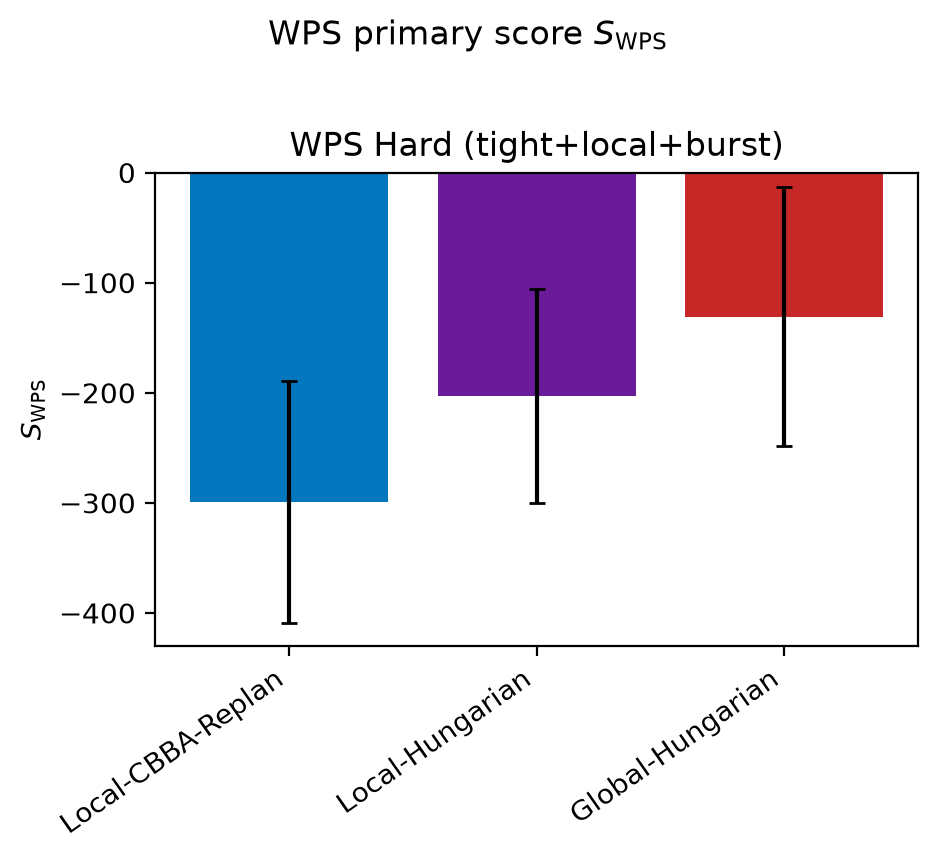
\includegraphics[width=\columnwidth]{figures/fig_wps_swps.png}
\caption{Primary \(S_{\mathrm{WPS}}\) across WPS suites (100 episodes).}
\label{fig:swps}
\end{figure}

\begin{figure}[t]
\centering
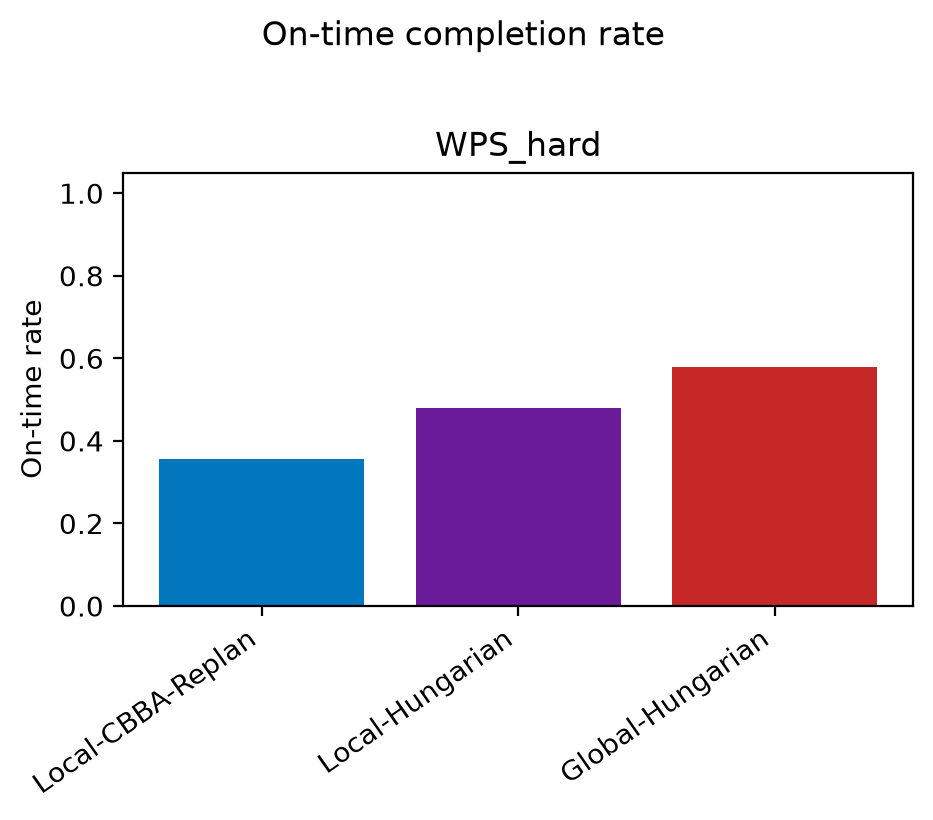
\includegraphics[width=\columnwidth]{figures/fig_wps_ontime.png}
\caption{On-time completion rate across suites.}
\label{fig:ontime}
\end{figure}

\subsection{Cross-suite behavior}
On \textbf{WPS\_easy}, Local-Hungarian achieves the best \(S_{\mathrm{WPS}}\) (\(24.4\)); hybrids do not beat it---myopic matching already fits soft delay.
On \textbf{WPS\_burst}, Att-RAH matches Local-Hungarian; the no-priority ablation (\(S_{\mathrm{WPS}}=-178.7\)) is competitive, suggesting engineered urgency/scarcity carries much of the signal under extreme stress.

\begin{figure}[t]
\centering
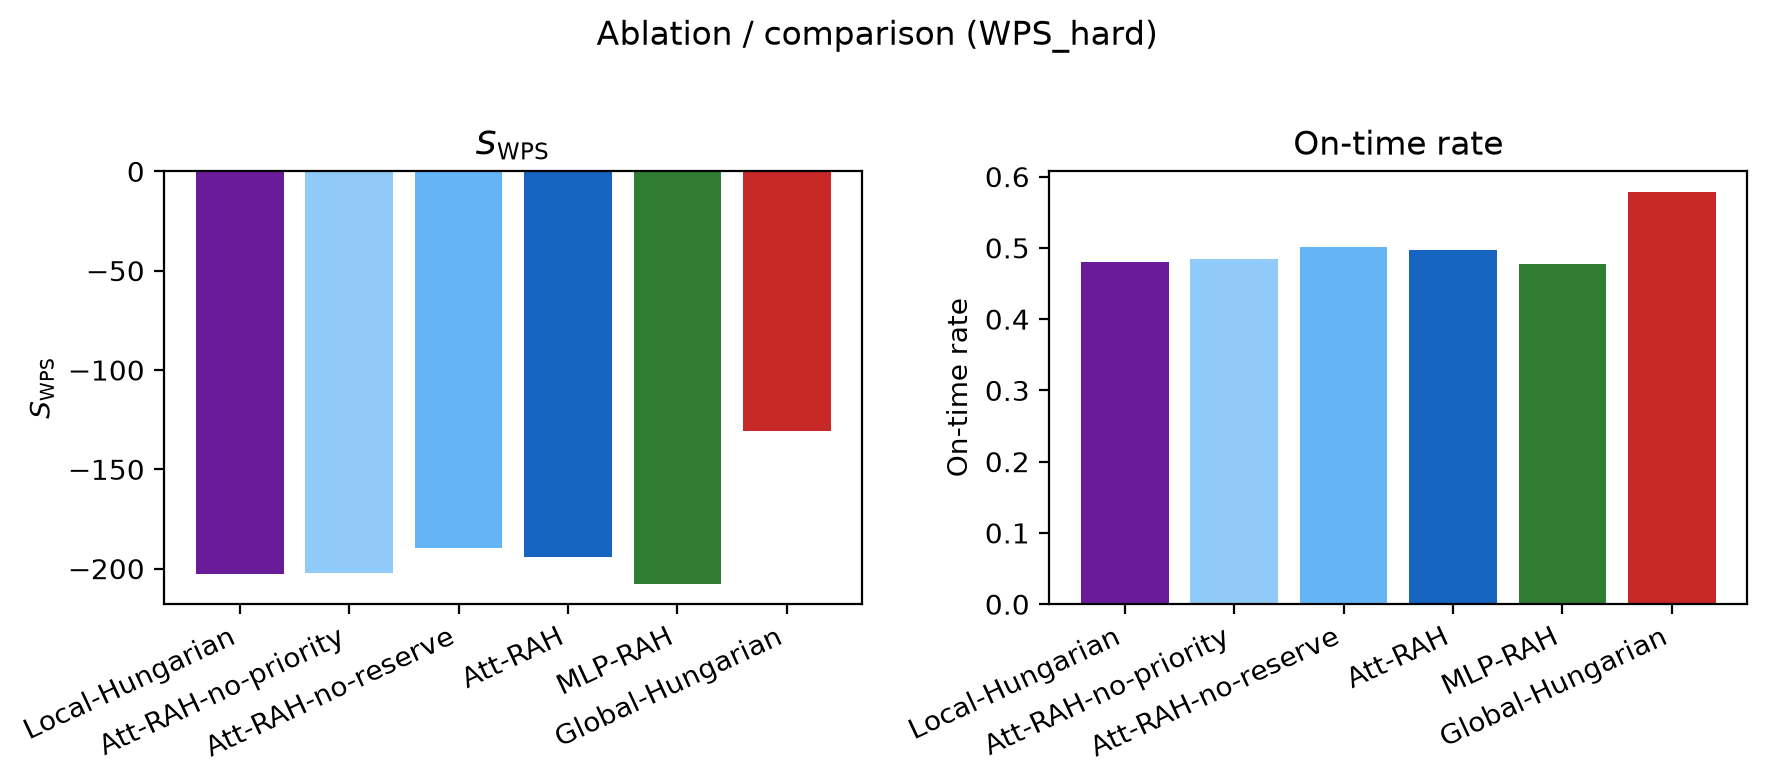
\includegraphics[width=\columnwidth]{figures/fig_wps_ablation.png}
\caption{Ablation panel on WPS\_hard: reserve is weak; hybrids approach but do not reach the oracle.}
\label{fig:ablation}
\end{figure}

\begin{figure}[t]
\centering
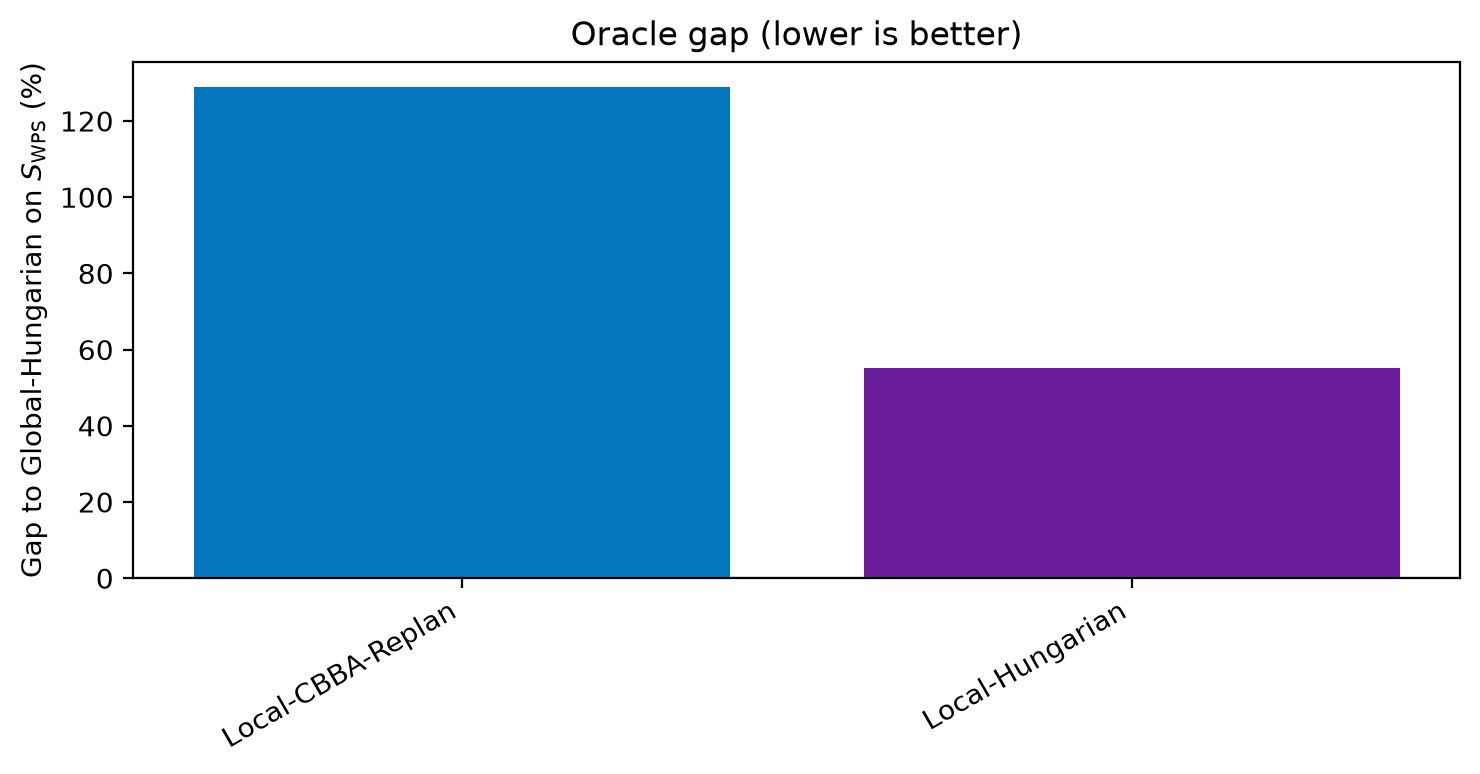
\includegraphics[width=\columnwidth]{figures/fig_wps_oracle_gap.png}
\caption{Relative gap to Global-Hungarian on \(S_{\mathrm{WPS}}\) (WPS\_hard).}
\label{fig:gap}
\end{figure}

\subsection{Ablations (WPS\_hard)}
Removing reserve does not hurt (and slightly helps mean \(S_{\mathrm{WPS}}\)).
Removing the learned priority head but keeping urgency/scarcity still beats Local-Hungarian on hard.
Att-RAH's CI vs Local excludes zero; MLP-RAH's does not under the same budget.

\subsection{Attention stress suite (WPS\_attn)}
To test whether set attention helps under stronger asymmetry, we evaluate a 12-UAV multi-front suite with dual-region bursts, scarce F2 specialists, and \emph{no} team knowledge sharing (discovery only via sensing radius).

\begin{table}[t]
\centering
\caption{WPS\_attn (100 eps). Attention does not separate from Local-Hungarian / ablations.}
\label{tab:attn}
\setlength{\tabcolsep}{3pt}
\begin{tabular}{lcccc}
\toprule
Method & \(S_{\mathrm{WPS}}\) & on-time & miss & \(\Delta S\) 95\% CI \\
\midrule
CBBA-Replan & $-413.6\pm116$ & 0.33 & 17.2 & $[-123,-74]$ \\
Local-Hung. & $-316.1\pm124$ & 0.43 & 15.0 & --- \\
MLP-RAH & $-313.8\pm110$ & 0.43 & 14.9 & $[-21,+25]$ \\
Att-RAH & $-316.5\pm122$ & 0.42 & 15.0 & $[-23,+23]$ \\
Att no-res. & $-313.1\pm126$ & 0.43 & 14.9 & $[-17,+23]$ \\
Att no-pri. & $-309.9\pm119$ & 0.43 & 14.8 & $[-7,+21]$ \\
Global (oracle) & $-166.7\pm83$ & 0.56 & 11.5 & $[+125,+174]$ \\
\bottomrule
\end{tabular}
\end{table}

Att-RAH does not beat Local-Hungarian, MLP-RAH, or the urgency/scarcity-only ablation (all CIs include zero).
The oracle gap grows (\(\approx 150\) \(S_{\mathrm{WPS}}\)), confirming that \emph{information}, not encoder depth, dominates under this hybrid interface.

\begin{figure}[t]
\centering
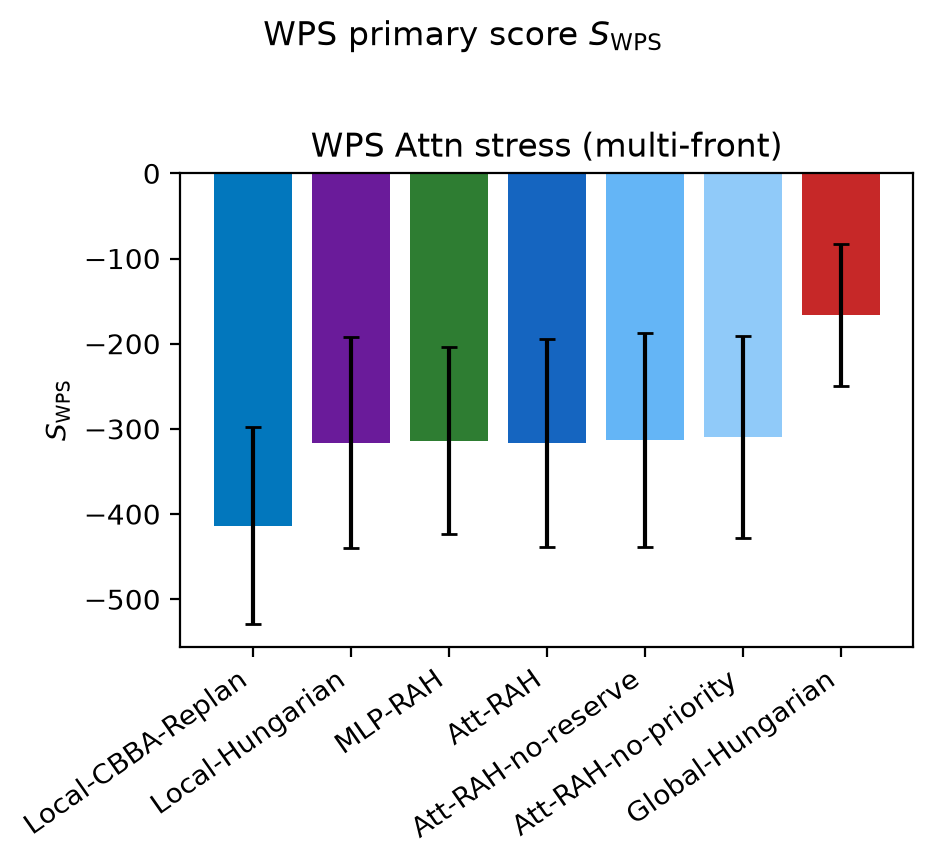
\includegraphics[width=\columnwidth]{figures/fig_wps_attn_swps.png}
\caption{WPS\_attn \(S_{\mathrm{WPS}}\): hybrids collapse to Local-Hungarian; Global remains far ahead.}
\label{fig:attn}
\end{figure}

\section{Discussion}
The results support a scoped claim: \emph{on WPS\_hard, hybrid cost shaping can significantly improve \(S_{\mathrm{WPS}}\) over myopic Local-Hungarian}.
Reserve is empirically weak.
Set attention is not a free lunch: when the policy only outputs priorities into Hungarian, richer scenes mainly enlarge the information gap to Global-Hungarian without rewarding deeper encoders.
Future work should change the decision interface (e.g., joint multi-agent commitments, learned communication, or rolling-horizon plans) if the goal is to demonstrate attention-specific gains.

\section{Conclusion}
We reformulated multi-UAV TA evaluation around WPS dynamics and \(S_{\mathrm{WPS}}\).
Att-RAH significantly improves over Local-Hungarian on WPS\_hard, while a multi-front stress suite shows that attention does not automatically outperform urgency heuristics or an MLP under the same hybrid assignment engine.
Code, checkpoints, and figure pipelines accompany the paper for Overleaf/GitHub reproduction.

\section*{Acknowledgments}
Omitted for anonymous review.

\bibliographystyle{IEEEtran}
\bibliography{refs}

\end{document}
